\documentclass[a4paper,10pt]{article}
\usepackage[utf8]{inputenc}
\usepackage[T1]{fontenc}
\usepackage[provide=*,french]{babel}
\usepackage{lmodern}
\usepackage[left=0.62cm,right=0.62cm,top=0.42cm,bottom=1.10cm]{geometry}
\usepackage{tikz}
\usepackage{graphicx}
\usepackage{xcolor}
\usepackage{eso-pic}
\usepackage{amssymb}
\usetikzlibrary{calc,arrows.meta}
\pagestyle{empty}
\renewcommand{\familydefault}{\sfdefault}
\setlength{\parindent}{0pt}

% Couleurs maths&go, identiques au gabarit du théorème direct.
\definecolor{brandNavy}{RGB}{11,53,112}
\definecolor{brandBlue}{RGB}{17,70,140}
\definecolor{brandTeal}{RGB}{29,174,174}
\definecolor{brandOrange}{RGB}{255,145,20}
\definecolor{softBlue}{RGB}{225,238,255}
\definecolor{softTeal}{RGB}{219,247,246}
\definecolor{softOrange}{RGB}{255,238,215}
\definecolor{softGreen}{RGB}{224,246,229}
\definecolor{softGray}{RGB}{245,247,250}
\definecolor{lightLine}{RGB}{190,230,230}

\newcommand{\LogoFile}{../assets/img/mathsgo-logo.png}
\newcommand{\MathsGoFooter}{%
\begin{tikzpicture}[remember picture,overlay]
  \node[anchor=south west,inner sep=0pt] at ([xshift=0.48cm,yshift=0.44cm]current page.south west)
    {\IfFileExists{\LogoFile}{\includegraphics[width=2.45cm]{\LogoFile}}{}};
  \node[anchor=south,text=brandNavy!70,font=\sffamily\bfseries\fontsize{7}{7}\selectfont]
    at ([yshift=0.32cm]current page.south) {mathsgo.re \textperiodcentered\ CC BY-NC-SA 4.0};
\end{tikzpicture}%
}
\AddToShipoutPictureFG{\MathsGoFooter}

\newcommand{\LowDotted}[1]{%
\begin{tikzpicture}[baseline=-0.78ex]
  \draw[densely dotted,line width=0.95pt,line cap=round] (0,-0.22) -- (#1,-0.22);
\end{tikzpicture}}
\newcommand{\StepBadge}[1]{\tikz[baseline=-0.62ex]{\node[circle,fill=brandNavy,text=white,font=\bfseries,minimum size=0.60cm,inner sep=0pt]{#1};}}
\newcommand{\StepHead}[2]{\StepBadge{#1}\hspace{0.20cm}{\bfseries\color{brandNavy}\fontsize{13.6}{14.4}\selectfont #2}}
\newcommand{\CheckBox}{\ensuremath{\Box}\,}
\newcommand{\Sep}{\vspace{0.12cm}\noindent\textcolor{lightLine}{\rule{19.3cm}{0.42pt}}\vspace{0.12cm}}

\newcommand{\TermColorBox}[3]{\tikz[baseline=-0.72ex]{\node[rounded corners=4pt,draw=#1,fill=#2,line width=0.78pt,inner xsep=5pt,inner ysep=4.5pt,minimum width=2.35cm,minimum height=0.72cm,font=\bfseries\fontsize{12.7}{13.4}\selectfont\color{brandNavy}]{#3};}}
\newcommand{\TermH}[1]{\TermColorBox{brandTeal}{softGreen}{#1}}
\newcommand{\TermB}[1]{\TermColorBox{brandBlue}{softBlue}{#1}}
\newcommand{\TermO}[1]{\TermColorBox{brandOrange}{softOrange}{#1}}
\newcommand{\TermN}[1]{\TermColorBox{brandNavy!45}{softGray}{#1}}

% Triangle quelconque : aucun angle droit n'est codé avant la conclusion.
\newcommand{\ReciprocalFigure}[1]{%
\begin{tikzpicture}[scale=#1,line join=miter,line cap=round]
  \coordinate (A) at (0,0);
  \coordinate (B) at (0.40,1.15);
  \coordinate (C) at (1.50,0);
  % Carré sur AB : bleu.
  \filldraw[fill=softBlue,draw=brandNavy,line width=0.85pt]
    (A) -- (B) -- (-0.75,1.55) -- (-1.15,0.40) -- cycle;
  % Carré sur AC : orange.
  \filldraw[fill=softOrange,draw=brandNavy,line width=0.85pt]
    (C) -- (A) -- (0,-1.50) -- (1.50,-1.50) -- cycle;
  % Carré sur BC, le plus grand côté : vert.
  \filldraw[fill=softGreen,draw=brandNavy,line width=0.85pt]
    (B) -- (C) -- (2.65,1.10) -- (1.55,2.25) -- cycle;
  \filldraw[fill=white,draw=brandNavy,line width=1.15pt] (A) -- (B) -- (C) -- cycle;
  \node[brandNavy!55,font=\bfseries\small] at (-0.16,-0.16) {$\cdots$};
  \node[brandNavy!55,font=\bfseries\small] at (0.27,1.33) {$\cdots$};
  \node[brandNavy!55,font=\bfseries\small] at (1.67,-0.15) {$\cdots$};
  \node[brandTeal,font=\bfseries\Large] at (0.25,0.23) {?};
\end{tikzpicture}}

\newcommand{\CompareBar}[3]{%
\begin{tikzpicture}[x=1cm,y=1cm]
  \def\W{7.80}\def\H{0.78}
  \draw[rounded corners=1pt,fill=softGreen,draw=brandNavy!80,line width=0.85pt] (0,\H) rectangle (\W,{2*\H});
  \node[font=\bfseries\fontsize{12.5}{13.2}\selectfont\color{brandNavy}] at ({\W/2},{1.5*\H}) {#1};
  \draw[rounded corners=1pt,fill=softBlue,draw=brandNavy!80,line width=0.85pt] (0,0) rectangle (3.30,\H);
  \draw[rounded corners=1pt,fill=softOrange,draw=brandNavy!80,line width=0.85pt] (3.30,0) rectangle (\W,\H);
  \node[font=\bfseries\fontsize{12.5}{13.2}\selectfont\color{brandNavy}] at (1.65,{0.5*\H}) {#2};
  \node[font=\bfseries\fontsize{12.5}{13.2}\selectfont\color{brandNavy}] at (5.55,{0.5*\H}) {#3};
\end{tikzpicture}}

\newcommand{\HeaderReciproque}{%
\noindent\begin{minipage}[c]{0.43\textwidth}
  \centering \ReciprocalFigure{1.58}
\end{minipage}%
\hfill
\begin{minipage}[c]{0.55\textwidth}
  \begin{center}
  {\fontsize{28}{29}\selectfont\bfseries\color{brandNavy} Réciproque du}\par\vspace{-0.01cm}
  {\fontsize{28}{29}\selectfont\bfseries\color{brandNavy} théorème de Pythagore}\par\vspace{0.12cm}
  {\fontsize{11.4}{12.5}\selectfont\bfseries\color{brandTeal} Objectif : déterminer si un triangle est rectangle à partir de ses trois longueurs.}\par\vspace{0.16cm}
  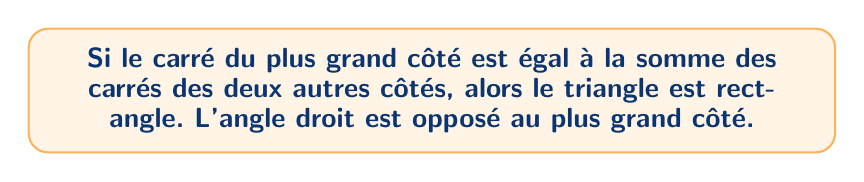
\begin{tikzpicture}
  \node[rounded corners=7pt,draw=brandOrange!70,fill=softOrange!65,line width=0.75pt,text width=9.75cm,inner sep=7pt,align=center,font=\bfseries\fontsize{9.9}{10.9}\selectfont\color{brandNavy}] {Si le carré du plus grand côté est égal à la somme des carrés des deux autres côtés, alors le triangle est rectangle. L'angle droit est opposé au plus grand côté.};
  \end{tikzpicture}
  \end{center}
\end{minipage}\par\vspace{0.42cm}}

\begin{document}

% ================= PAGE 1 : outil de décision =================
\HeaderReciproque

\StepHead{1}{Je complète ma figure et j'identifie le plus grand côté}\par\vspace{0.14cm}
{\small\bfseries\color{brandNavy} Je nomme les sommets et j'indique les trois longueurs. Je surligne le plus grand côté. Je ne l'appelle pas encore hypoténuse : je ne sais pas encore si le triangle est rectangle.}\par\vspace{0.28cm}

\StepHead{2}{Je calcule séparément les deux quantités}\par\vspace{0.13cm}
{\fontsize{10.8}{11.7}\selectfont Dans le triangle \LowDotted{2.25}, le plus grand côté est \LowDotted{1.55}.}\par\vspace{0.18cm}
\noindent\begin{minipage}[t]{8.95cm}
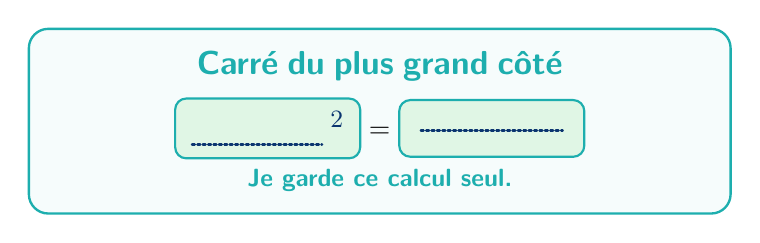
\begin{tikzpicture}
\node[rounded corners=7pt,draw=brandTeal,fill=brandTeal!4,line width=0.85pt,text width=8.35cm,inner sep=8pt,align=center] {
{\bfseries\color{brandTeal}\fontsize{11.5}{12.3}\selectfont Carré du plus grand côté}\par\vspace{0.18cm}
\TermH{$\LowDotted{1.65}^{\;2}$}\;=\;\TermH{$\LowDotted{1.80}$}\par\vspace{0.09cm}
{\fontsize{9.3}{10.1}\selectfont\bfseries\color{brandTeal} Je garde ce calcul seul.}
};
\end{tikzpicture}
\end{minipage}\hfill
\begin{minipage}[t]{9.95cm}
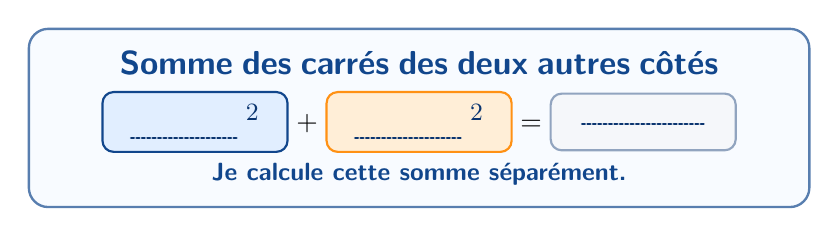
\begin{tikzpicture}
\node[rounded corners=7pt,draw=brandBlue!70,fill=softBlue!22,line width=0.85pt,text width=9.35cm,inner sep=8pt,align=center] {
{\bfseries\color{brandBlue}\fontsize{11.5}{12.3}\selectfont Somme des carrés des deux autres côtés}\par\vspace{0.18cm}
\TermB{$\LowDotted{1.35}^{\;2}$}\;+\;\TermO{$\LowDotted{1.35}^{\;2}$}\;=\;\TermN{$\LowDotted{1.55}$}\par\vspace{0.09cm}
{\fontsize{9.3}{10.1}\selectfont\bfseries\color{brandBlue} Je calcule cette somme séparément.}
};
\end{tikzpicture}
\end{minipage}

\vspace{0.12cm}
\begin{center}
\CompareBar{$\LowDotted{2.15}$}{$\LowDotted{1.55}$}{$\LowDotted{2.05}$}
\end{center}
\Sep

\StepHead{3}{Je compare les deux résultats}\par\vspace{0.13cm}
\begin{center}

\begin{tikzpicture}
\node[rounded corners=7pt,draw=brandNavy!45,fill=white,line width=0.85pt,text width=13.7cm,inner sep=8pt,align=center] {
\TermH{$\LowDotted{2.05}$}\quad
\tikz[baseline=-0.55ex]{\node[draw=brandNavy!55,rounded corners=4pt,fill=softGray,minimum width=1.45cm,minimum height=0.72cm,font=\bfseries\Large\color{brandNavy}] {$=$ ou $\neq$};}
\quad\TermN{$\LowDotted{2.05}$}\par\vspace{0.10cm}
{\fontsize{9.8}{10.6}\selectfont\bfseries\color{brandNavy} Je compare les nombres obtenus, pas les longueurs de départ.}
};
\end{tikzpicture}
\end{center}

\StepHead{4}{Je choisis le bon chemin}\par\vspace{0.13cm}
\noindent\begin{minipage}[t]{9.35cm}
{\bfseries\color{brandTeal}\fontsize{11.8}{12.6}\selectfont \CheckBox Les deux résultats sont égaux}\par\vspace{0.06cm}
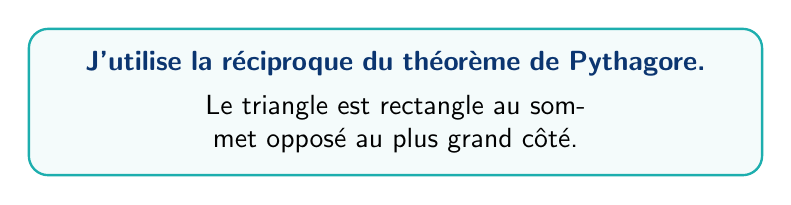
\begin{tikzpicture}
\node[rounded corners=7pt,draw=brandTeal,fill=brandTeal!5,line width=0.85pt,text width=8.75cm,inner sep=8pt,align=center] {
{\bfseries\color{brandNavy} J'utilise la réciproque du théorème de Pythagore.}\par\vspace{0.14cm}
Le triangle est rectangle au sommet opposé au plus grand côté.
};
\end{tikzpicture}
\end{minipage}\hfill
\begin{minipage}[t]{9.35cm}
{\bfseries\color{brandOrange}\fontsize{11.8}{12.6}\selectfont \CheckBox Les deux résultats sont différents}\par\vspace{0.06cm}

\begin{tikzpicture}
\node[rounded corners=7pt,draw=brandOrange,fill=brandOrange!5,line width=0.85pt,text width=8.75cm,inner sep=8pt,align=center] {
{\bfseries\color{brandNavy} J'utilise la contraposée du théorème de Pythagore.}\par\vspace{0.14cm}
Le triangle n'est pas rectangle.
};
\end{tikzpicture}
\end{minipage}

\vspace{0.20cm}
\StepHead{5}{Je rédige ma conclusion}\par\vspace{0.12cm}
\begin{center}
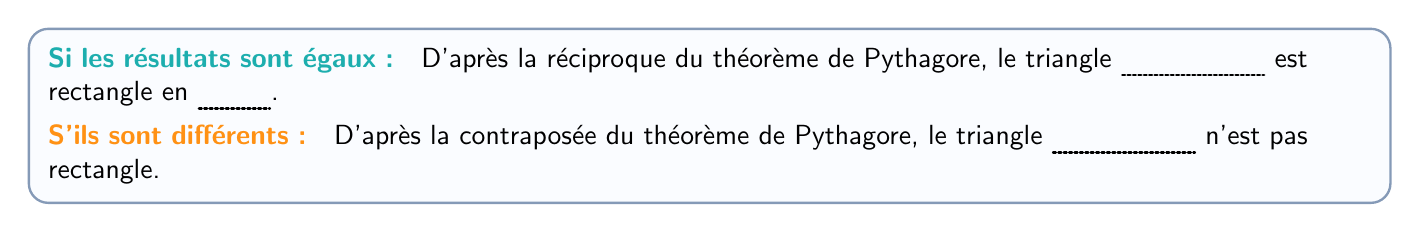
\begin{tikzpicture}
\node[rounded corners=7pt,draw=brandNavy!50,fill=softBlue!16,line width=0.85pt,text width=16.8cm,inner sep=7pt,align=left] {
{\bfseries\color{brandTeal} Si les résultats sont égaux :}\quad D'après la réciproque du théorème de Pythagore, le triangle \LowDotted{1.80} est \mbox{rectangle} en \LowDotted{0.90}.\par\vspace{0.14cm}
{\bfseries\color{brandOrange} S'ils sont différents :}\quad D'après la contraposée du théorème de Pythagore, le triangle \LowDotted{1.80} n'est pas \mbox{rectangle}.
};
\end{tikzpicture}
\end{center}

\vspace{0.02cm}
\begin{center}

\begin{tikzpicture}
\node[rounded corners=7pt,fill=softOrange!55,draw=brandOrange!55,line width=0.6pt,text width=16.9cm,inner sep=5pt,align=center] {\small\bfseries\color{brandNavy} Je vérifie : ai-je comparé le carré du plus grand côté avec la somme des carrés des deux autres côtés ? \hspace{0.22cm}$\Box$ oui \hspace{0.18cm}$\Box$ non};
\end{tikzpicture}
\end{center}

\newpage

% ================= PAGE 2 : rédaction propre =================
\begin{center}
{\fontsize{26}{28}\selectfont\bfseries\color{brandNavy} Réciproque du théorème de Pythagore}\par\vspace{0.04cm}
{\fontsize{15}{16}\selectfont\bfseries\color{brandTeal} Rédaction propre pour déterminer si un triangle est rectangle}
\end{center}\vspace{0.18cm}

\noindent
\begin{minipage}[t]{5.70cm}
\vspace{0pt}
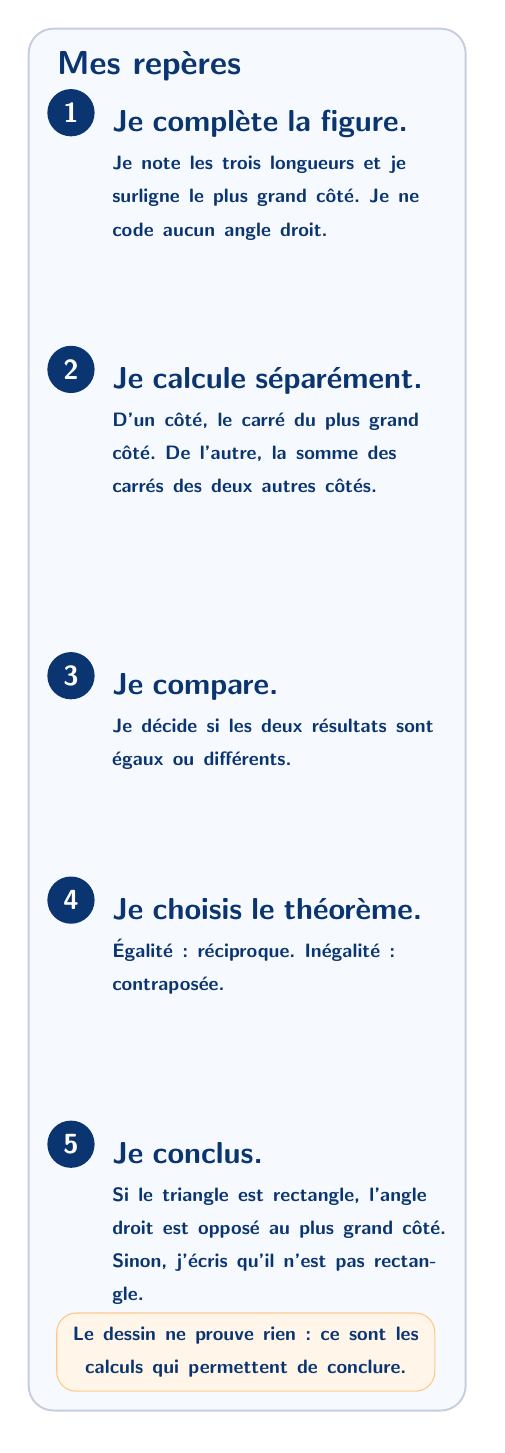
\begin{tikzpicture}[x=1cm,y=1cm]
\path[use as bounding box] (0,0) rectangle (5.70,-17.75);
\node[rounded corners=9pt,draw=brandNavy!24,fill=softBlue!30,line width=0.70pt,minimum width=5.55cm,minimum height=17.55cm,anchor=north west] at (0,0) {};
\node[anchor=north west,text=brandNavy,font=\bfseries\fontsize{12.6}{13.6}\selectfont] at (0.25,-0.18) {Mes repères};

\node[circle,fill=brandNavy,text=white,font=\bfseries,minimum size=0.60cm,inner sep=0pt] at (0.55,-1.08) {1};
\node[anchor=north west,text width=4.30cm,align=left] at (0.95,-0.93) {\bfseries\color{brandNavy}\fontsize{11.1}{11.9}\selectfont Je complète la figure.\par\vspace{0.06cm}
{\scriptsize\bfseries\color{brandNavy} Je note les trois longueurs et je surligne le plus grand côté. Je ne code aucun angle droit.}};

\node[circle,fill=brandNavy,text=white,font=\bfseries,minimum size=0.60cm,inner sep=0pt] at (0.55,-4.34) {2};
\node[anchor=north west,text width=4.30cm,align=left] at (0.95,-4.19) {\bfseries\color{brandNavy}\fontsize{11.1}{11.9}\selectfont Je calcule séparément.\par\vspace{0.06cm}
{\scriptsize\bfseries\color{brandNavy} D'un côté, le carré du plus grand côté. De l'autre, la somme des carrés des deux autres côtés.}};

\node[circle,fill=brandNavy,text=white,font=\bfseries,minimum size=0.60cm,inner sep=0pt] at (0.55,-8.23) {3};
\node[anchor=north west,text width=4.30cm,align=left] at (0.95,-8.08) {\bfseries\color{brandNavy}\fontsize{11.1}{11.9}\selectfont Je compare.\par\vspace{0.06cm}
{\scriptsize\bfseries\color{brandNavy} Je décide si les deux résultats sont égaux ou différents.}};

\node[circle,fill=brandNavy,text=white,font=\bfseries,minimum size=0.60cm,inner sep=0pt] at (0.55,-11.08) {4};
\node[anchor=north west,text width=4.30cm,align=left] at (0.95,-10.93) {\bfseries\color{brandNavy}\fontsize{11.1}{11.9}\selectfont Je choisis le théorème.\par\vspace{0.06cm}
{\scriptsize\bfseries\color{brandNavy} Égalité : réciproque. Inégalité : contraposée.}};

\node[circle,fill=brandNavy,text=white,font=\bfseries,minimum size=0.60cm,inner sep=0pt] at (0.55,-14.18) {5};
\node[anchor=north west,text width=4.30cm,align=left] at (0.95,-14.03) {\bfseries\color{brandNavy}\fontsize{11.1}{11.9}\selectfont Je conclus.\par\vspace{0.06cm}
{\scriptsize\bfseries\color{brandNavy} Si le triangle est rectangle, l'angle droit est opposé au plus grand côté. Sinon, j'écris qu'il n'est pas rectangle.}};

\node[rounded corners=7pt,draw=brandOrange!50,fill=softOrange!55,text width=4.45cm,inner sep=5pt,align=center] at (2.77,-16.82) {\scriptsize\bfseries\color{brandNavy} Le dessin ne prouve rien : ce sont les calculs qui permettent de conclure.};
\end{tikzpicture}
\end{minipage}\hfill
\begin{minipage}[t]{13.05cm}
\vspace{0pt}
{\bfseries\color{brandTeal}\fontsize{10.8}{11.4}\selectfont Je surligne le plus grand côté, sans dessiner d'angle droit.}\par\vspace{0.06cm}
\begin{center}
\begin{tikzpicture}
\node[rounded corners=8pt,draw=brandTeal!65,fill=brandTeal!3,line width=0.75pt,text width=12.25cm,inner sep=7pt,align=center] {
% sharp corners : le « rounded corners=8pt » du cadre englobant est hérité par
% cette figure et arrondissait les sommets du triangle.
% Proportions 3-4-5 (AB = 2, AC = 2,75, BC = 3,4) : BC est nettement le plus
% grand côté ; l'angle en A vaut environ 88°, il n'est pas codé.
\begin{tikzpicture}[x=1.2cm,y=1.2cm,line cap=butt,line join=miter,sharp corners]
  \coordinate (A) at (0,0); \coordinate (B) at (0.22,2.00); \coordinate (C) at (2.75,-0.18);
  \fill[white] (A) -- (B) -- (C) -- cycle;
  \draw[brandTeal,line width=4.5pt,opacity=.24] (B) -- (C);
  \draw[brandNavy,line width=1.25pt] (A) -- (B) -- (C) -- cycle;
  % Noms des sommets (A en bas à gauche, B en haut, C à droite).
  \node[brandNavy!70,font=\bfseries\small] at (-0.30,-0.28) {\LowDotted{0.65}};
  \node[brandNavy!70,font=\bfseries\small] at (0.22,2.28) {\LowDotted{0.65}};
  \node[brandNavy!70,font=\bfseries\small] at (3.12,-0.42) {\LowDotted{0.65}};
  % Longueurs : AB à gauche, AC en dessous, BC au-dessus du surlignage.
  \node[brandNavy!70,font=\bfseries\small] at (-0.42,1.00) {\LowDotted{0.85}};
  \node[brandNavy!70,font=\bfseries\small] at (1.38,-0.50) {\LowDotted{0.85}};
  \node[brandTeal,font=\bfseries\small] at (1.88,1.30) {\LowDotted{0.85}};
\end{tikzpicture}
};
\end{tikzpicture}
\end{center}

\vspace{0.08cm}
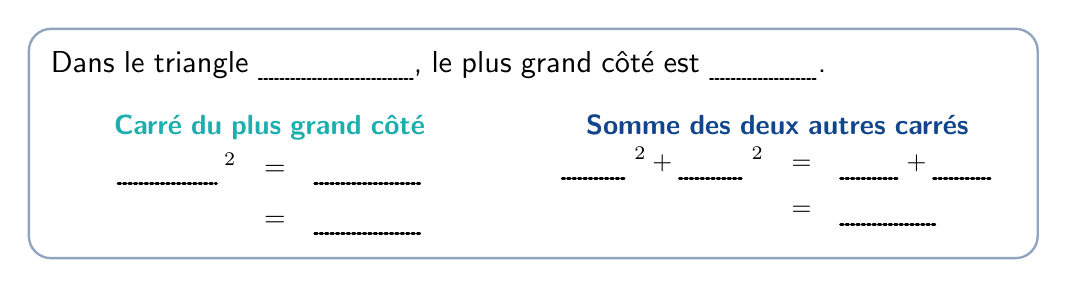
\begin{tikzpicture}
\node[rounded corners=8pt,draw=brandNavy!45,fill=white,line width=0.85pt,text width=12.25cm,inner sep=8pt,align=left] {
{\fontsize{10.5}{11.8}\selectfont Dans le triangle \LowDotted{1.95}, le plus grand côté est \LowDotted{1.35}.}\par\vspace{0.13cm}
\noindent\begin{minipage}[t]{5.55cm}
\centering{\bfseries\color{brandTeal} Carré du plus grand côté}\par\vspace{0.12cm}
$\begin{array}{rcl}
\LowDotted{1.25}^{\;2} & = & \LowDotted{1.35}\\[0.22cm]
                       & = & \LowDotted{1.35}
\end{array}$
\end{minipage}\hfill
\begin{minipage}[t]{6.05cm}
\centering{\bfseries\color{brandBlue} Somme des deux autres carrés}\par\vspace{0.12cm}
{\fontsize{9.4}{10.2}\selectfont$\begin{array}{rcl}
\LowDotted{0.82}^{\;2}+\LowDotted{0.82}^{\;2} & = & \LowDotted{0.75}+\LowDotted{0.75}\\[0.22cm]
                                                & = & \LowDotted{1.20}
\end{array}$}
\end{minipage}
};
\end{tikzpicture}

\vspace{0.18cm}
\begin{center}

\begin{tikzpicture}
\node[rounded corners=7pt,draw=brandNavy!45,fill=softGray,line width=0.8pt,text width=10.8cm,inner sep=7pt,align=center] {
{\bfseries\color{brandNavy} Je compare les deux résultats}\par\vspace{0.12cm}
\TermH{$\LowDotted{1.70}$}\quad $=$ ou $\neq$ \quad\TermN{$\LowDotted{1.70}$}
};
\end{tikzpicture}
\end{center}

\vspace{0.10cm}
\noindent\begin{minipage}[t]{6.18cm}
{\bfseries\color{brandTeal}\fontsize{11.2}{12.0}\selectfont \CheckBox Les résultats sont égaux}\par\vspace{0.06cm}
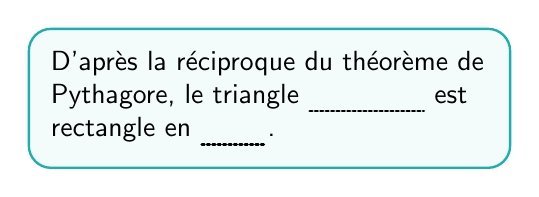
\begin{tikzpicture}
\node[rounded corners=8pt,draw=brandTeal,fill=brandTeal!5,line width=0.85pt,text width=5.55cm,inner sep=8pt,align=left] {
{\fontsize{10.0}{11.3}\selectfont D'après la réciproque du théorème de Pythagore, le triangle \LowDotted{1.45} est rectangle en \LowDotted{0.82}.}
};
\end{tikzpicture}
\end{minipage}\hfill
\begin{minipage}[t]{6.18cm}
{\bfseries\color{brandOrange}\fontsize{11.2}{12.0}\selectfont \CheckBox Les résultats sont différents}\par\vspace{0.06cm}
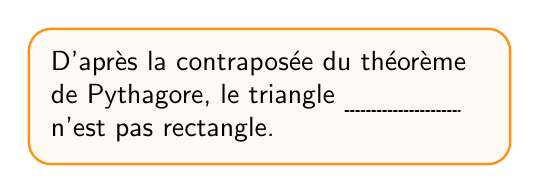
\begin{tikzpicture}
\node[rounded corners=8pt,draw=brandOrange,fill=brandOrange!5,line width=0.85pt,text width=5.55cm,inner sep=8pt,align=left] {
{\fontsize{10.0}{11.3}\selectfont D'après la contraposée du théorème de Pythagore, le triangle \LowDotted{1.45} n'est pas rectangle.}
};
\end{tikzpicture}
\end{minipage}

\vspace{0.32cm}
\begin{center}
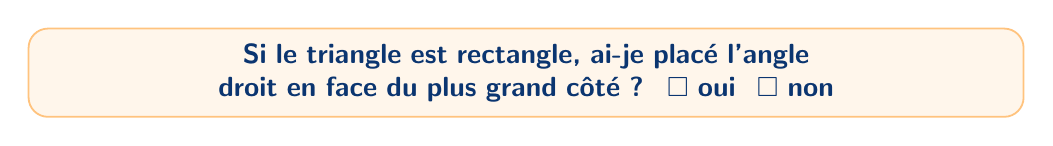
\begin{tikzpicture}
\node[rounded corners=7pt,draw=brandOrange!55,fill=softOrange!50,line width=0.65pt,text width=12.25cm,inner sep=5.5pt,align=center] {\bfseries\color{brandNavy} Si le triangle est rectangle, ai-je placé l'angle droit en face du plus grand côté ? \hspace{0.18cm}$\Box$ oui \hspace{0.15cm}$\Box$ non};
\end{tikzpicture}
\end{center}

\vspace{0.30cm}
{\bfseries\color{brandNavy}\fontsize{12.2}{13.0}\selectfont Deux exemples pour vérifier mon raisonnement}\par\vspace{0.10cm}
\noindent\begin{minipage}[t]{6.18cm}
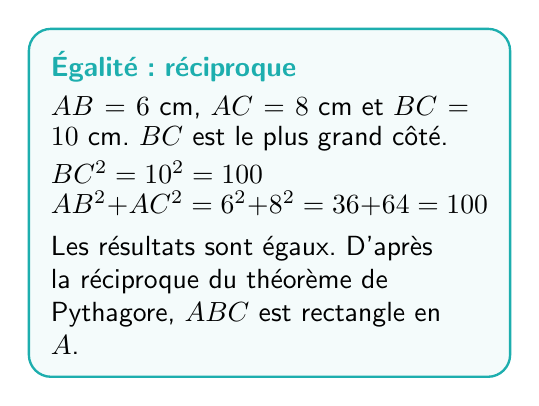
\begin{tikzpicture}
\node[rounded corners=8pt,draw=brandTeal,fill=brandTeal!5,line width=0.85pt,text width=5.55cm,minimum height=4.15cm,inner sep=8pt,align=left] {
{\bfseries\color{brandTeal} Égalité : réciproque}\par\vspace{0.11cm}
{\fontsize{9.7}{10.9}\selectfont $AB=6$ cm, $AC=8$ cm et $BC=10$ cm. $BC$ est le plus grand côté.\par\vspace{0.10cm}
$BC^2=10^2=100$\par
$AB^2+AC^2=6^2+8^2=36+64=100$\par\vspace{0.10cm}
Les résultats sont égaux. D'après la réciproque du théorème de Pythagore, $ABC$ est rectangle en $A$.}
};
\end{tikzpicture}
\end{minipage}\hfill
\begin{minipage}[t]{6.18cm}
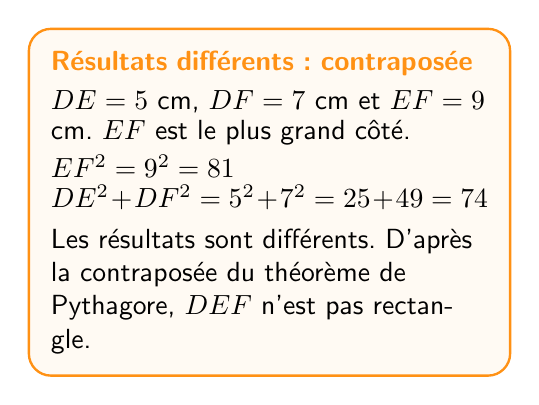
\begin{tikzpicture}
\node[rounded corners=8pt,draw=brandOrange,fill=brandOrange!5,line width=0.85pt,text width=5.55cm,minimum height=4.15cm,inner sep=8pt,align=left] {
{\bfseries\color{brandOrange} Résultats différents : contraposée}\par\vspace{0.11cm}
{\fontsize{9.7}{10.9}\selectfont $DE=5$ cm, $DF=7$ cm et $EF=9$ cm. $EF$ est le plus grand côté.\par\vspace{0.10cm}
$EF^2=9^2=81$\par
$DE^2+DF^2=5^2+7^2=25+49=74$\par\vspace{0.10cm}
Les résultats sont différents. D'après la contraposée du théorème de Pythagore, $DEF$ n'est pas rectangle.}
};
\end{tikzpicture}
\end{minipage}
\end{minipage}

\end{document}
